\section{Introduction}
This work aims to shed light on the representations learned by \textsf{Graph Neural Networks}. In this section, we will discuss the prevalence of graphs and the crucial role \gnns play in analyzing them. We will delve into the methods we use to gain insights and highlight the significance of our approach. Lastly, we will provide an overview of the structure of this work.

\subsection{Motivation}
Graphs are ubiquitous in various fields of life. Despite not always being explicitly identified as such, the graph data model's flexibility and simplicity make it an effective tool for modeling a diverse range of data. Examples of graph modeling applications include unexpected instances, such as modeling text or images as a graph, as well as more complex instances like chemical molecules, citation networks, or connectivity encodings of the World Wide Web \cite{Mor+2020, Sca+2009}.

Although machine learning has achieved remarkable success with image classification (e.g., \cite{Zoph2018, He2016}) and text generation (e.g., \cite{Radford2019, Brown2020}) in the last decade, the lack of a significant breakthrough in machine learning for graphs can be attributed to the graph data model's inherent flexibility and simplicity. While, for example, an image classifier constrains its input data to be a grid-like image or a text generator expects its input to be a linear sequence of words, machine learning models working on graphs cannot leverage any constraints on the format or size of their input graphs without limiting their generality. 

To put this flexibility of the graph data model into perspective and give an idea of how ubiquitous graphs are in various fields, we refer back to the examples of image classifiers and text generators and demonstrate how seemingly natural the graph data model can encode their input data. For example, images can be encoded by a graph, such that each pixel of the image corresponds to a node in the graph holding its color value, and each node is connected to its neighboring pixel nodes. Similarly, for sequential data like text files, one can encode a directed graph where each word in this file is represented as a node with the word as a feature and connected outgoingly to the next following word. See \cref{fig:example_encodings} for an illustrative example of these encodings.

In recent years, a significant amount of research has been conducted to investigate \textsf{Graph Neural Networks} (\gnns). Among the most promising approaches are those utilizing the message-passing architecture, which was introduced by \cite{Sca+2009} and \cite{Gil+2017}. 
Empirically, this framework has demonstrated strong performance across various applications \cite{Kip+2017, Ham+2017, Xu2018}. However, its expressiveness is limited, as has been proved by the works of \cite{Morris2018}, as well as \cite{Xu2018}. These works establish a connection to the \textsf{Weisfeiler-Leman}\footnote{Based on \href{https://www.iti.zcu.cz/wl2018/pdf/leman.pdf}{https://www.iti.zcu.cz/wl2018/pdf/leman.pdf}, we will use the spelling ``Leman'' here, as requested by A. Leman, the co-inventor of the algorithm.} algorithm (\wl), originally proposed by \cite{Wei+1968} as a simple heuristic for the graph isomorphism problem. In particular, it has been proven that a \gnn based on the message-passing architecture can, at most, be as good as the \wl algorithm in distinguishing non-isomorphic graphs. Furthermore, the \wl method demonstrates numerous similarities with the fundamental workings of the \gnn architecture. It is, therefore, commonly believed that both methods are, to some extent, equivalent in their capacity to capture information in a graph.

Despite the remarkable empirical performance of \gnns, particularly compared to conventional graph kernel functions \cite{Mor+2020}, and the theoretical understanding of their ability to distinguish non-isomorphic graphs, there remains a limited understanding of the learned representations that drive this empirical success. This work aims to delve into these representations, seeking deeper insights into the factors contributing to the efficacy of \gnns.

\begin{figure}[!t]
 \centering
 \begin{subfigure}[b]{0.475\textwidth}
    \centering
    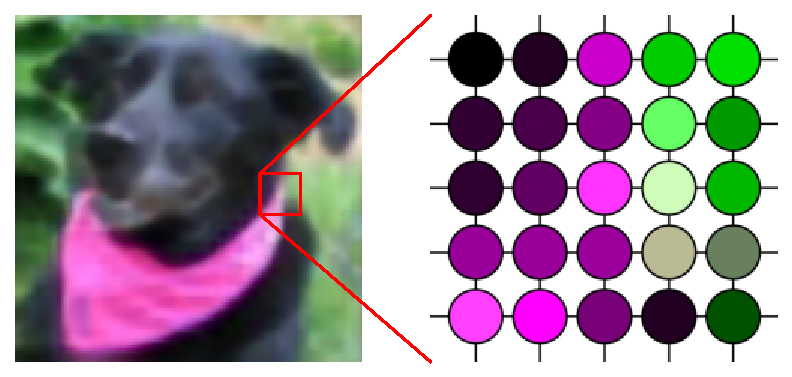
\includegraphics[width=\textwidth]{Figures/encoding_example.pdf}
    \caption{Graph Encoding of an Image\footnotemark}
 \end{subfigure}
 \hfill
 \begin{subfigure}[b]{0.475\textwidth}
    \centering
    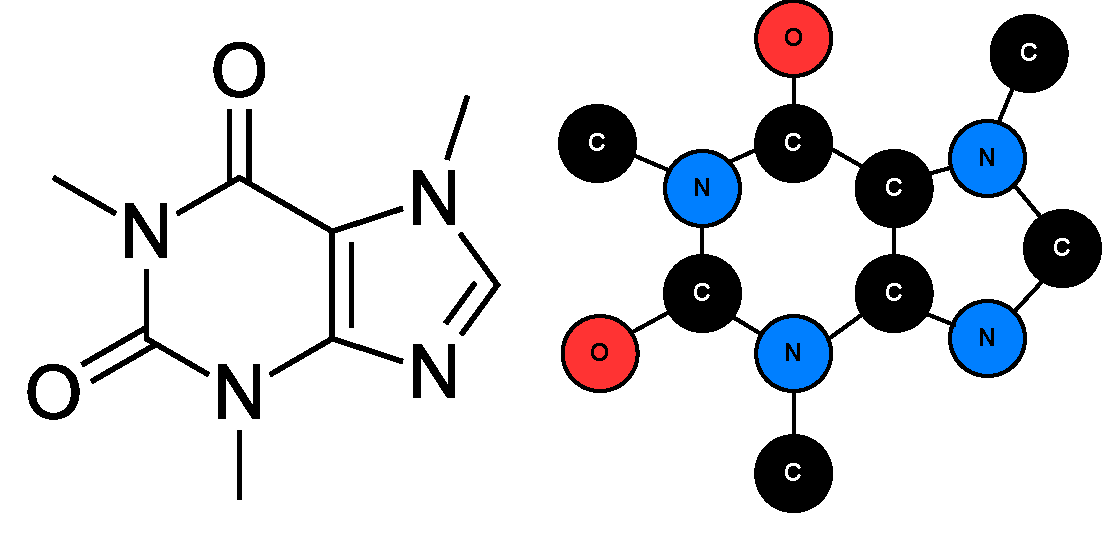
\includegraphics[width=\textwidth]{Figures/Example_Encoding_Molecule.pdf}
    \caption{Graph Encoding of a Molecule\footnotemark}
 \end{subfigure}
 \par\medskip
 \begin{subfigure}[b]{0.475\textwidth}
    \centering
    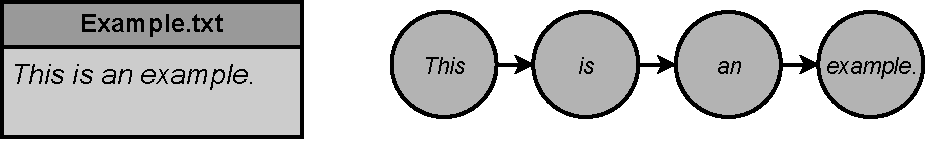
\includegraphics[width=\textwidth]{Figures/Example_Encoding_Text.pdf}
    \caption{Graph Encoding of a Text File.}
 \end{subfigure}
 \caption[Caption for LOF]{An overview of three examples of how graphs can be used to encode information across different domains. For each example, the conventional domain-specific encodings are visualized on the left, while on the right, we showcase how a graph can encode the same information. Note that these examples are just a sample; in actual practice, more detailed encodings are usually utilized to capture additional information.\footnotemark}
 \label{fig:example_encodings}
\end{figure}\todo{Footnotes are wrong!}
\footnotetext[2]{The image of a dog is from the CIFAR-10 collection made available by \cite{Krizhevsky2009}.}
\footnotetext[3]{The illustration of the skeletal formula of caffeine is taken from \href{https://commons.wikimedia.org/wiki/File:Caffeine_structure.svg}{https://commons.wikimedia.org}.}
\footnotetext{All graphics were created using the free open source platform \href{https://www.draw.io}{https://www.draw.io}.}

\subsection{Methology}
In this work, we introduce a novel framework, which we coined ``\wlnn,'' which involves applying the \wl algorithm to an input graph and further processing the resulting information using a feedforward neural network. Thereby, we obtain a trainable framework suited for all kinds of graph-related tasks, such as graph classification, node regression, and more. We will prove that both frameworks, \wlnn and \gnn, are theoretically equivalent, such that each function computed by a \wlnn model can also be computed by a \gnn model and vice versa. With this framework in hand, we can investigate the representations learned by a \gnn.

The interesting property of this framework compared to \gnns, which is also the original idea that inspired this work, is the fundamental difference in how both frameworks learn and optimize themselves when applied to a specific task. Take, for example, an arbitrary classification task. While the first part of a \wlnn model starts by applying the \wl algorithm to its input graph and retrieves a highly informative representation of this graph, the second part, the learnable feedforward neural network, must find common patterns in this very detailed representation that coincides with the class labels of the task, such that the model makes good predictions. In contrast, a \gnn first must learn how to process the information in a graph effectively and then find common patterns in its computed representation that correlate with the class labels so that the model can make good predictions.

To put both learning behaviors into perspective on a high level, while a \wlnn model is given a maximally informative representation and needs to find the essential information in this representation to make a good prediction, a \gnn works the other way around since it first has to learn how to effectively compute good representations of a graph and then leverage this information for good predictions. Despite their difference in learning behaviors, both methods can compute the same functions, making a fascinating comparison of their empirical performance.

Therefore, we will use this novel framework and various empirical experiments to compare both frameworks on multiple datasets to establish a deeper understanding of the representations learned by \gnns.

\subsection{Research Questions \& Contributions}
\begin{enumerate}
   \item \wlnn as a framework for analyzing \gnns. We will show the theoretical equivalence and show that both methods share many emprical similarities, such that this tool is a great for analyzing various aspects of a \gnn.
   \item We will show
\end{enumerate}

\subsection{Outline}
For ease of readability, we split this work into two parts. The first part investigates and establishes the theoretical equivalence between the frameworks of \wlnn and \gnns. In contrast, the second part presents our different experiments and their empirical results, in which we use the \wlnn framework as a tool to analyze the representation learned by a \gnn.

In detail, this work starts with \cref{sec:related_work}, where we discuss related work, milestones in \gnns over the past decade, essential properties of the \wl algorithm, and a subset of interesting connections between \gnns and the \wl algorithm.

Afterward, we will start with \cref{part1}, which begins with \cref{sec:pre_lim}. Here, we will introduce formal definitions for both frameworks, as well as a set of notations we will use throughout the theoretical part. Preceding, in \cref{sec:theo_connections}, we will introduce two theorems that each present a connection between both frameworks and combined prove the equivalence of both frameworks. Finally, we will prove each theorem individually after another in corresponding subsections.

The second part is dedicated to our empirical experiments. We begin with \cref{sec:testing_configuration}, explaining the experimental setup and our experiment choices. In detail, we will discuss the choice of benchmarking datasets, \gnn models, and \wlnn models, along with an explanation of our general testing procedure. In \cref{sec:emprical_results}, we present the results of our experiments and delve into further analyses of certain aspects of \gnn and \wlnn models. In particular, we will investigate the representations computed by \gnns and try to infer common patterns that occurred across multiple datasets. Finally, the thesis concludes with a final discussion in \cref{sec:discussion}, where we summarize our findings, address the limitations of this work, and offer recommendations for future research.